\subsection{Cuestionario 4}

\subsubsection{Pre-juego}
	
	 ¿Cuál es tu edad? \\
	Respuesta: El público en su mayoría que ha respondido la encuesta se encuentra entre los 21 y 25 años de edad y algunas personas entre los 30 y 40 años. \\ 
	
	 ¿Cuál es tú nivel de estudios? \\
	\begin{itemize}
		\item Básica
		\item Media superior
		\item Superior
		\item Doctorado o maestría
	\end{itemize}

\begin{figure}
	\centering
	\caption{Gráfica de nivel de estudios}
	\label{fig:pre01}
	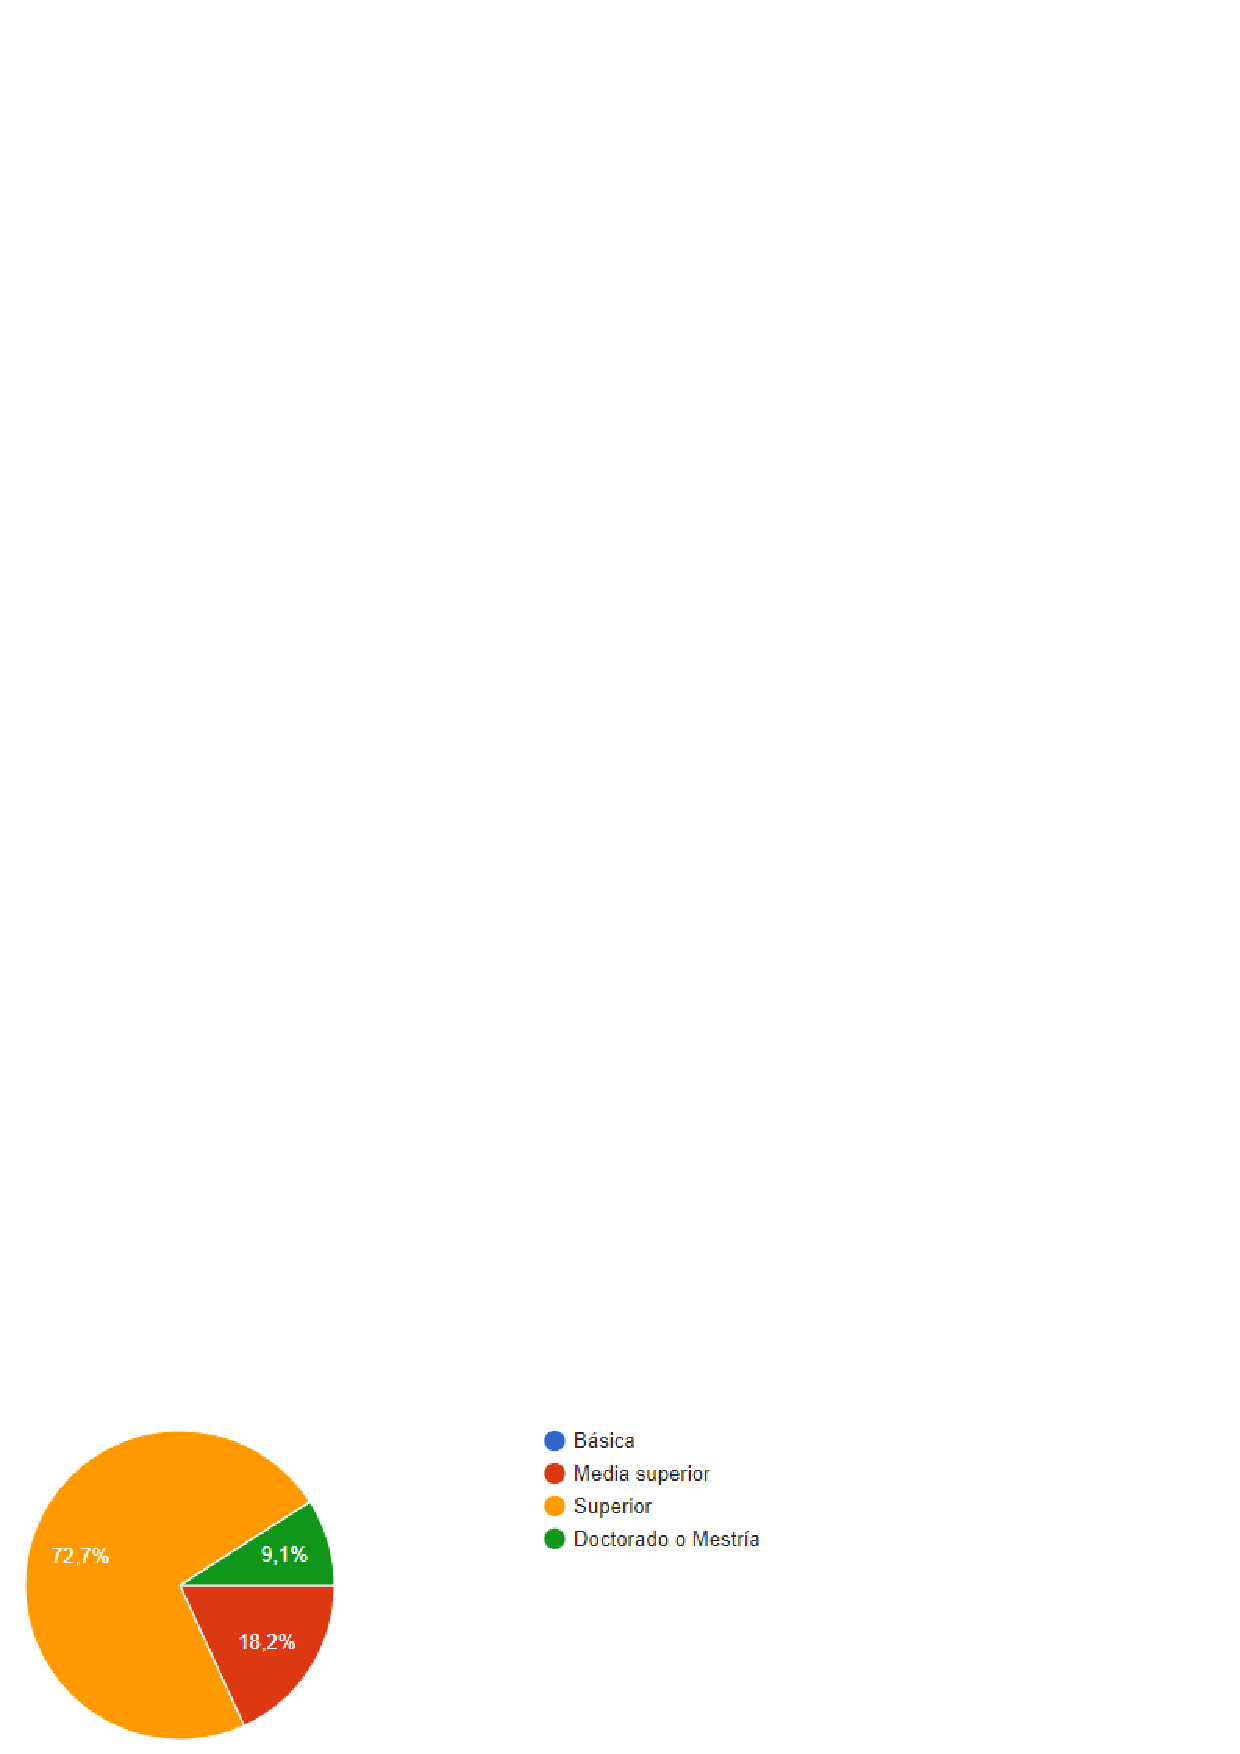
\includegraphics[width=0.5\textwidth]{04ResultadosObetnidos/pruebaR/imagenes/que/pre01}
\end{figure}

	
	 ¿Qué es lo primero que piensas cuando te dicen "cultura de México"?
	\begin{itemize}
		\item Comida
		\item Arquitectura o lugares
		\item Vestimenta
		\item Música
		\item Idioma	
	\end{itemize}

\begin{figure}
	\centering
	\caption{Gráfica de cultura de México}
	\label{fig:pre02}
	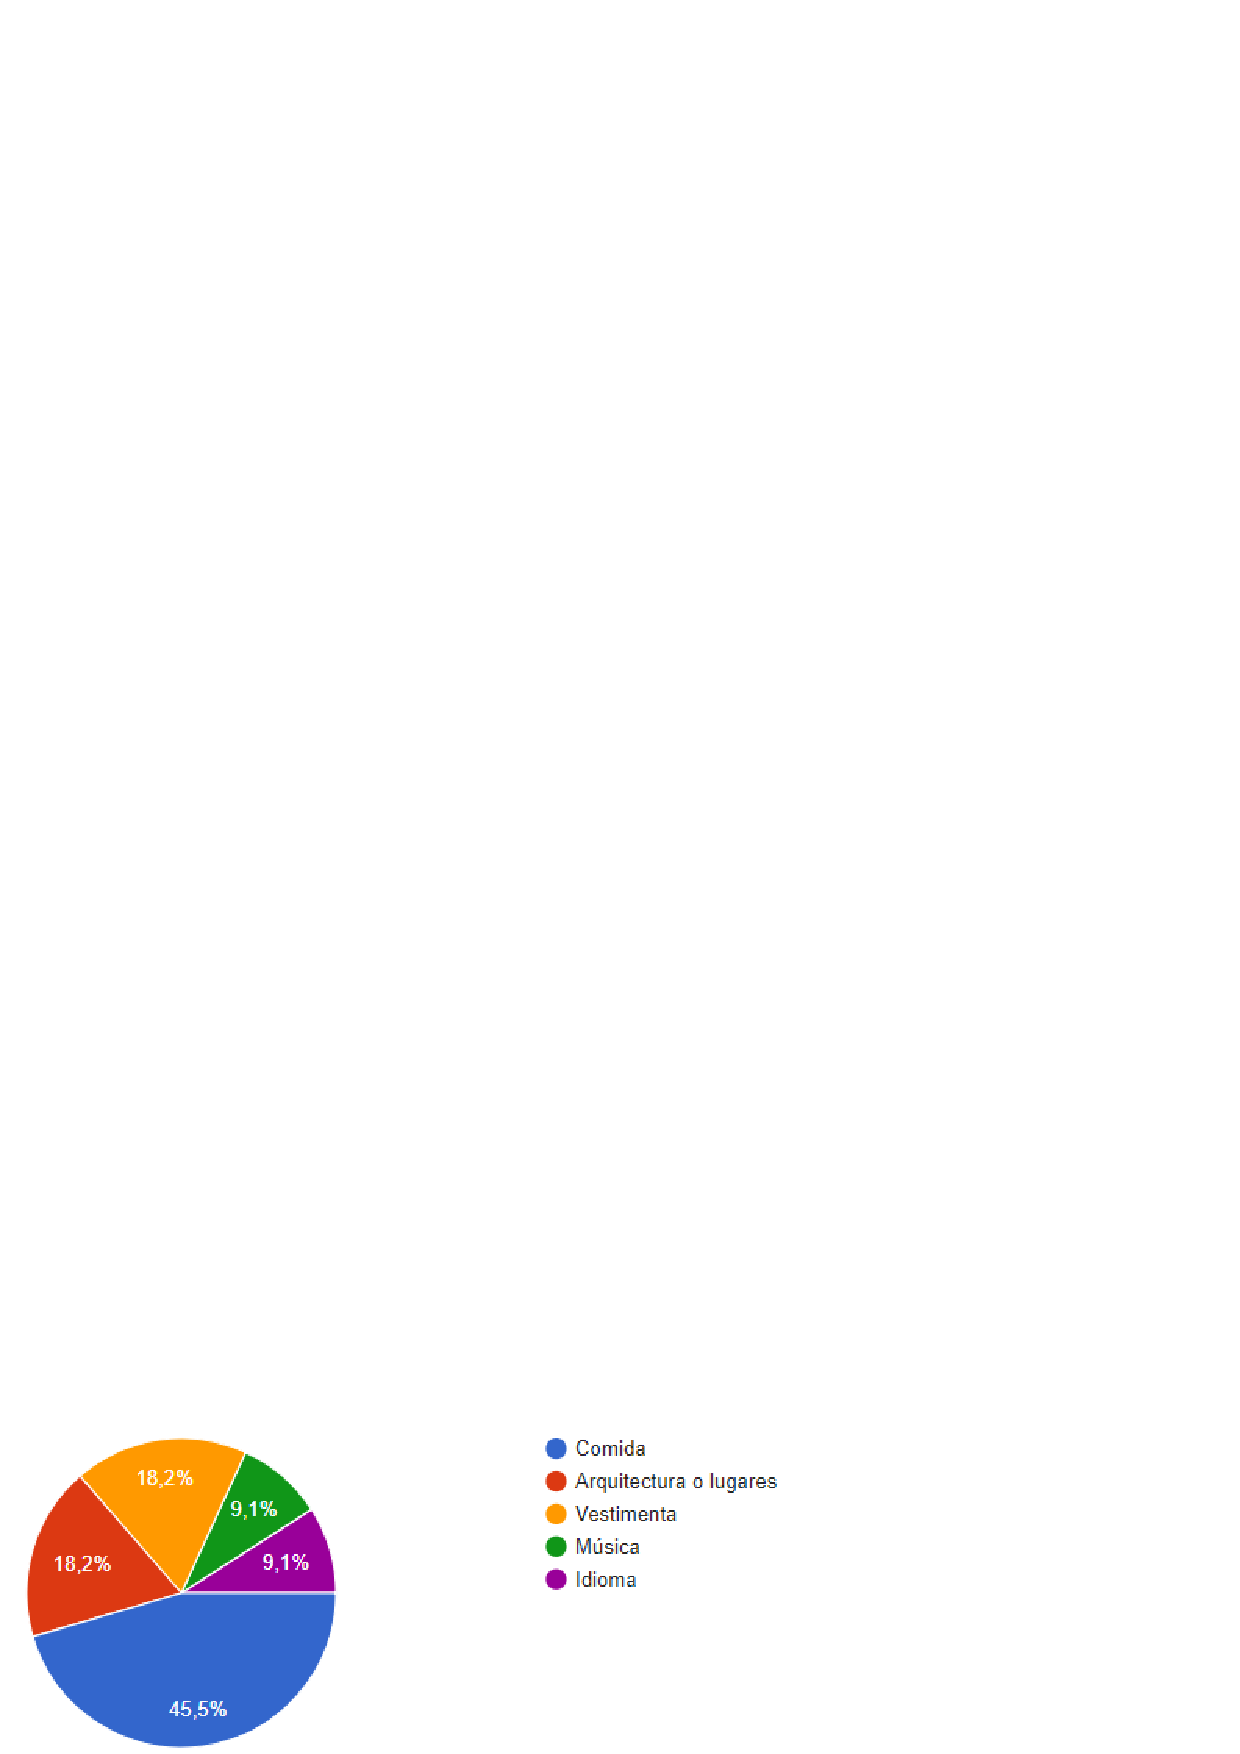
\includegraphics[width=0.5\textwidth]{04ResultadosObetnidos/pruebaR/imagenes/que/pre02}
\end{figure}

	
	¿Por qué motivos visitas lugares históricos?
	\begin{itemize}
		\item Escuela
		\item Trabajo
		\item Evento especial
		\item Interés propio
		\item Otro?
	\end{itemize}

\begin{figure}
	\centering
	\caption{Gráfica de lugares históricos}
	\label{fig:pre03}
	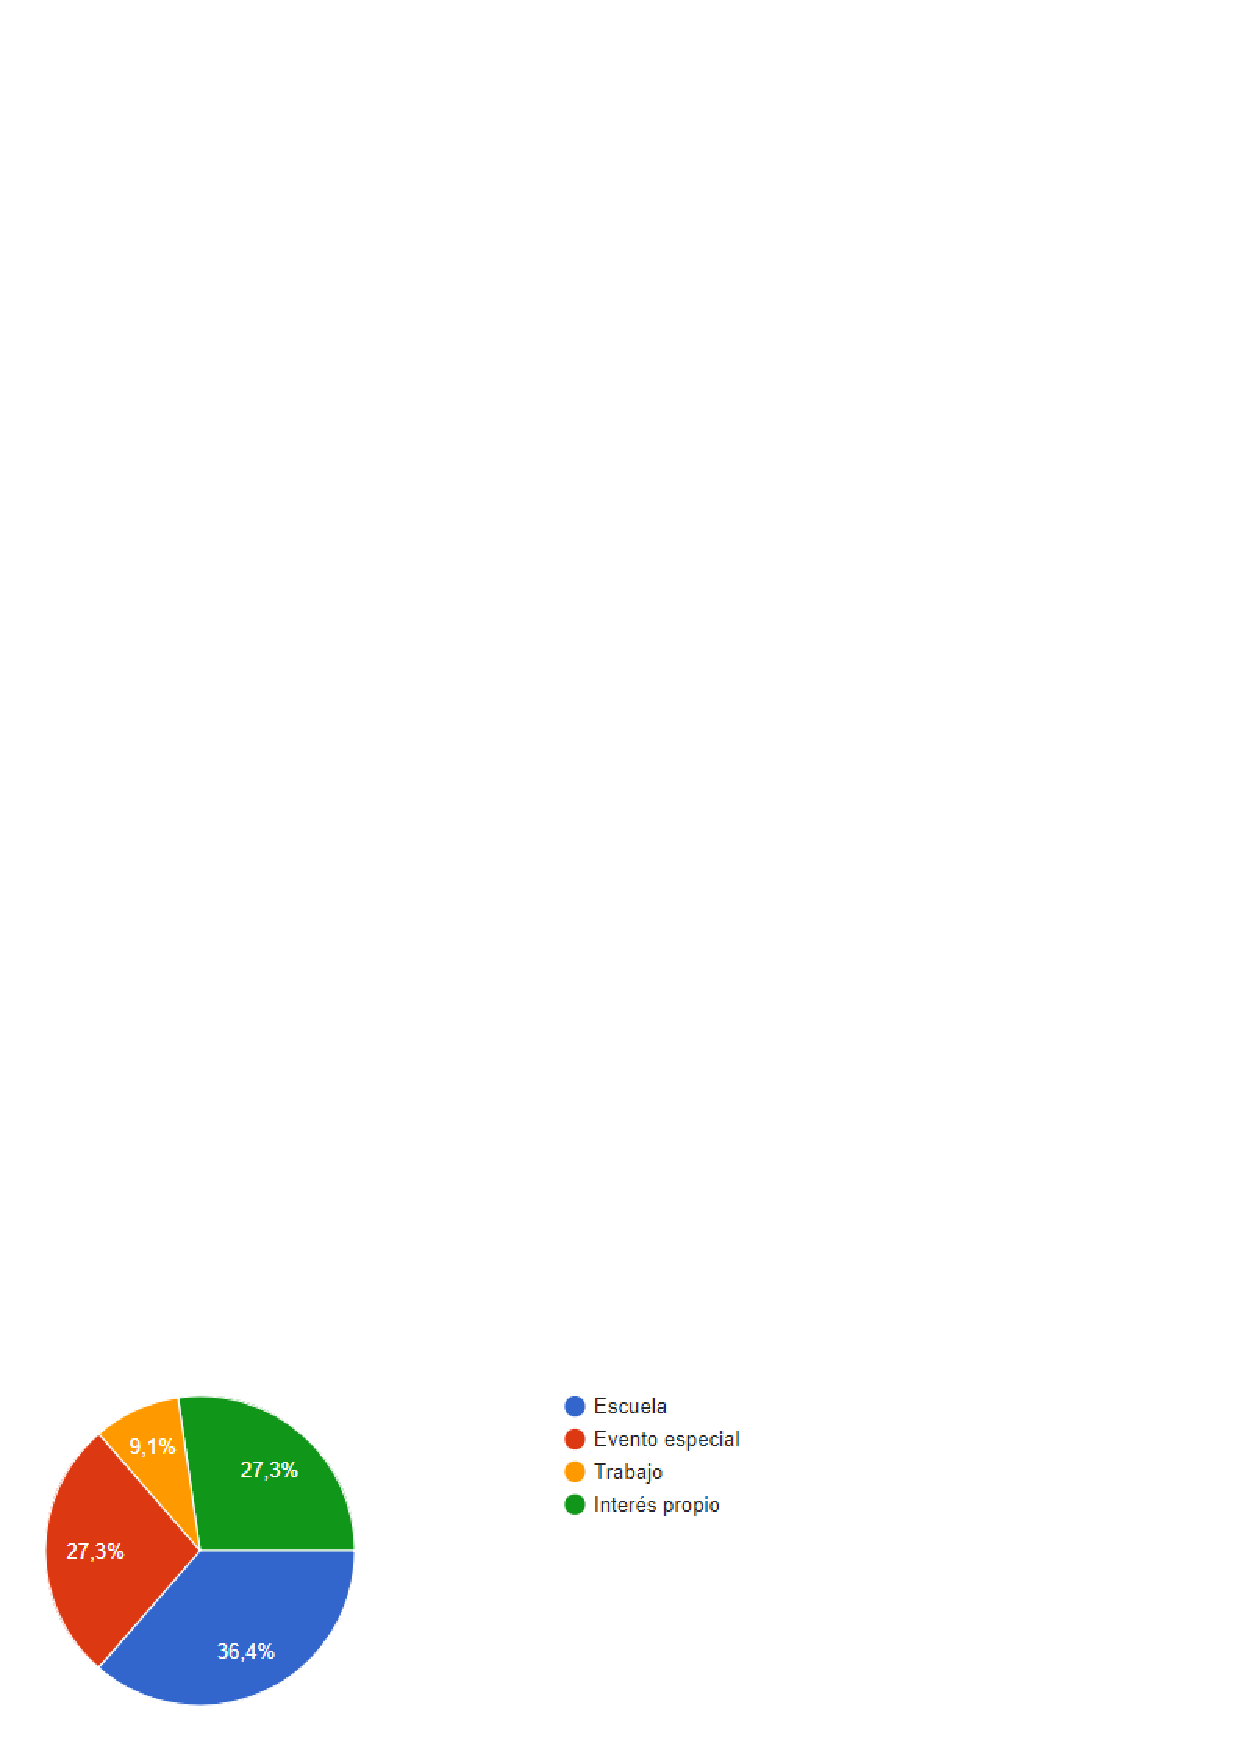
\includegraphics[width=0.5\textwidth]{04ResultadosObetnidos/pruebaR/imagenes/que/pre03}
\end{figure}

	
	¿Sabes sobre la cultura prehispánica en México?
	\begin{itemize}
		\item Sí
		\item No
		\item Creo
	\end{itemize}

\begin{figure}
	\centering
	\caption{Gráfica de cultura prehispánica}
	\label{fig:pre04}
	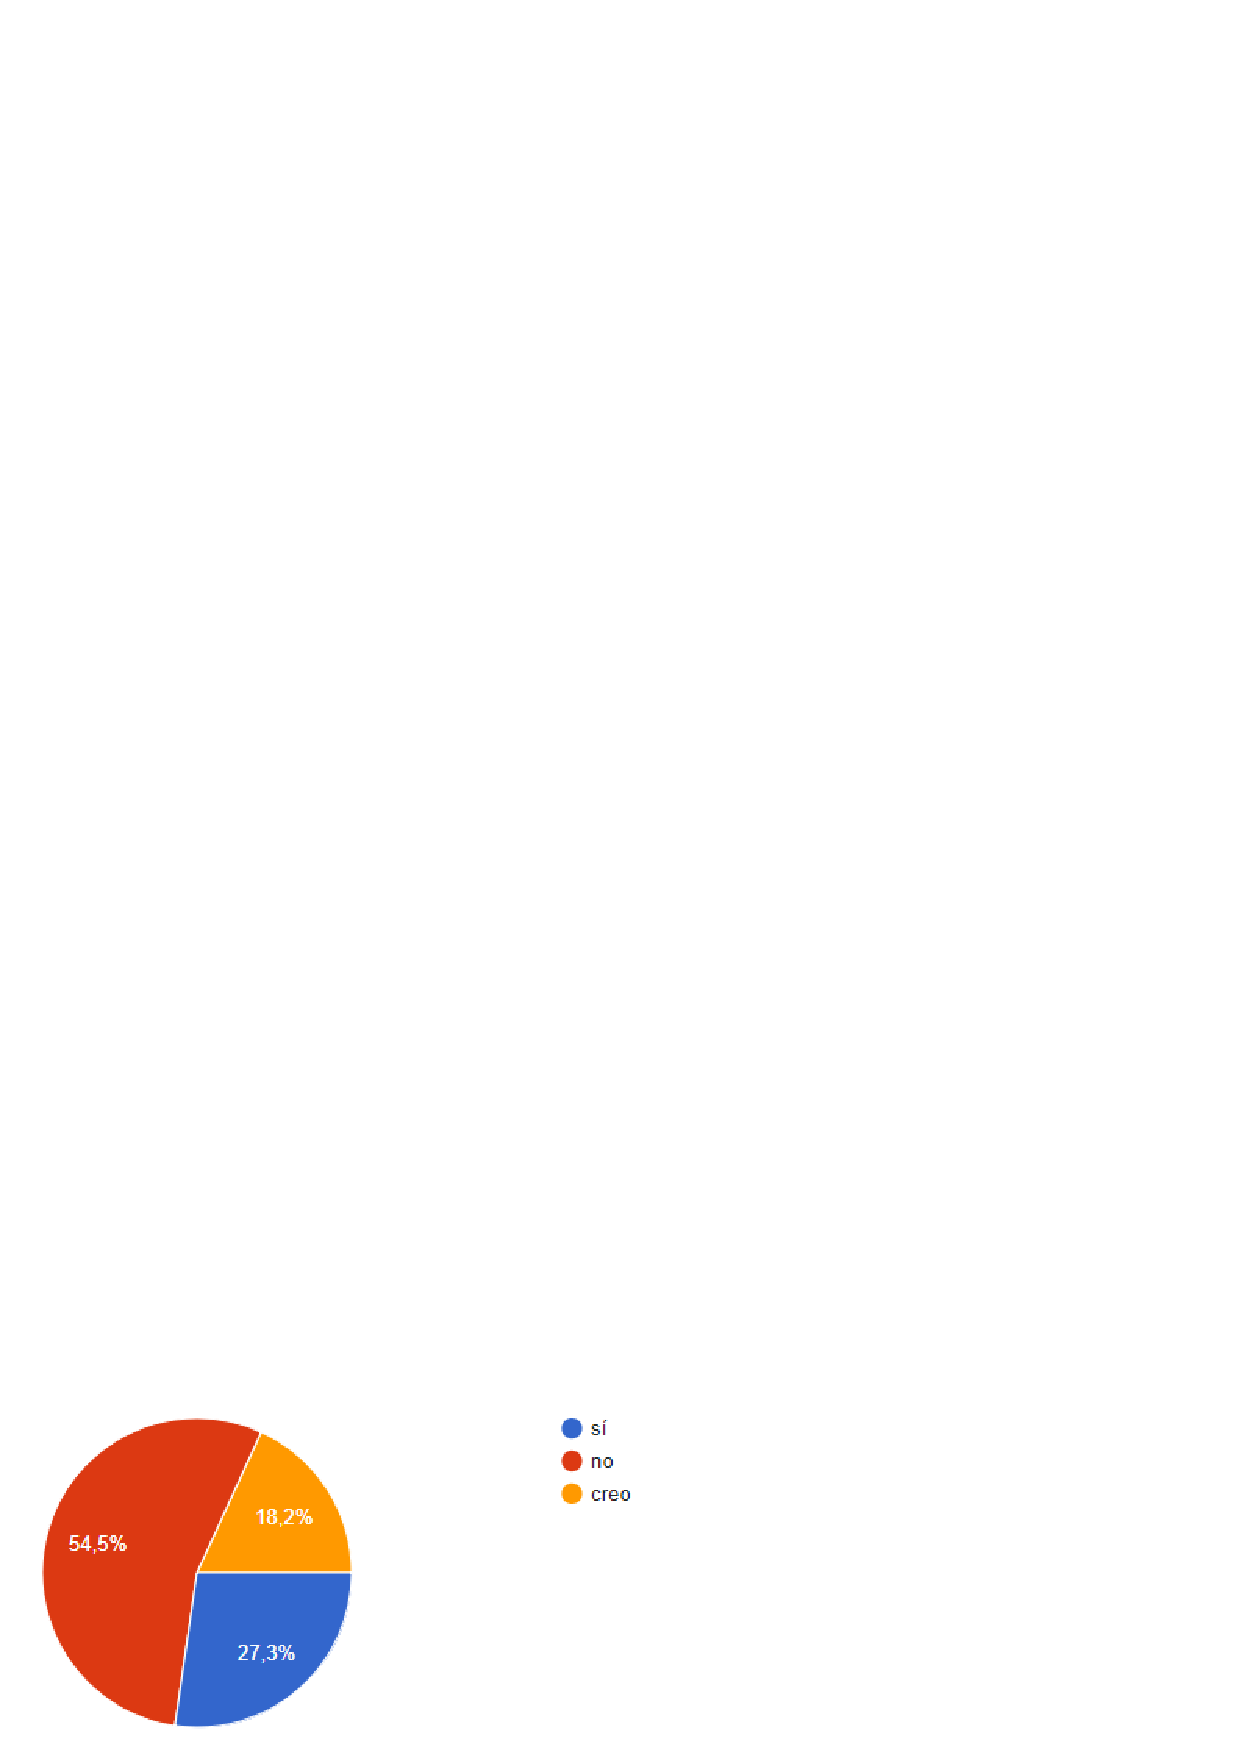
\includegraphics[width=0.5\textwidth]{04ResultadosObetnidos/pruebaR/imagenes/que/pre04}
\end{figure}

	
	¿Qué senitmiento tienes? 
	\begin{itemize}
		\item Alegría
		\item Enojo
		\item Tristeza
		\item Curiosidad
		\item Fatiga
		\item Otro?
	\end{itemize}

\begin{figure}
	\centering
	\caption{Gráfica de sentimiento}
	\label{fig:pre05}
	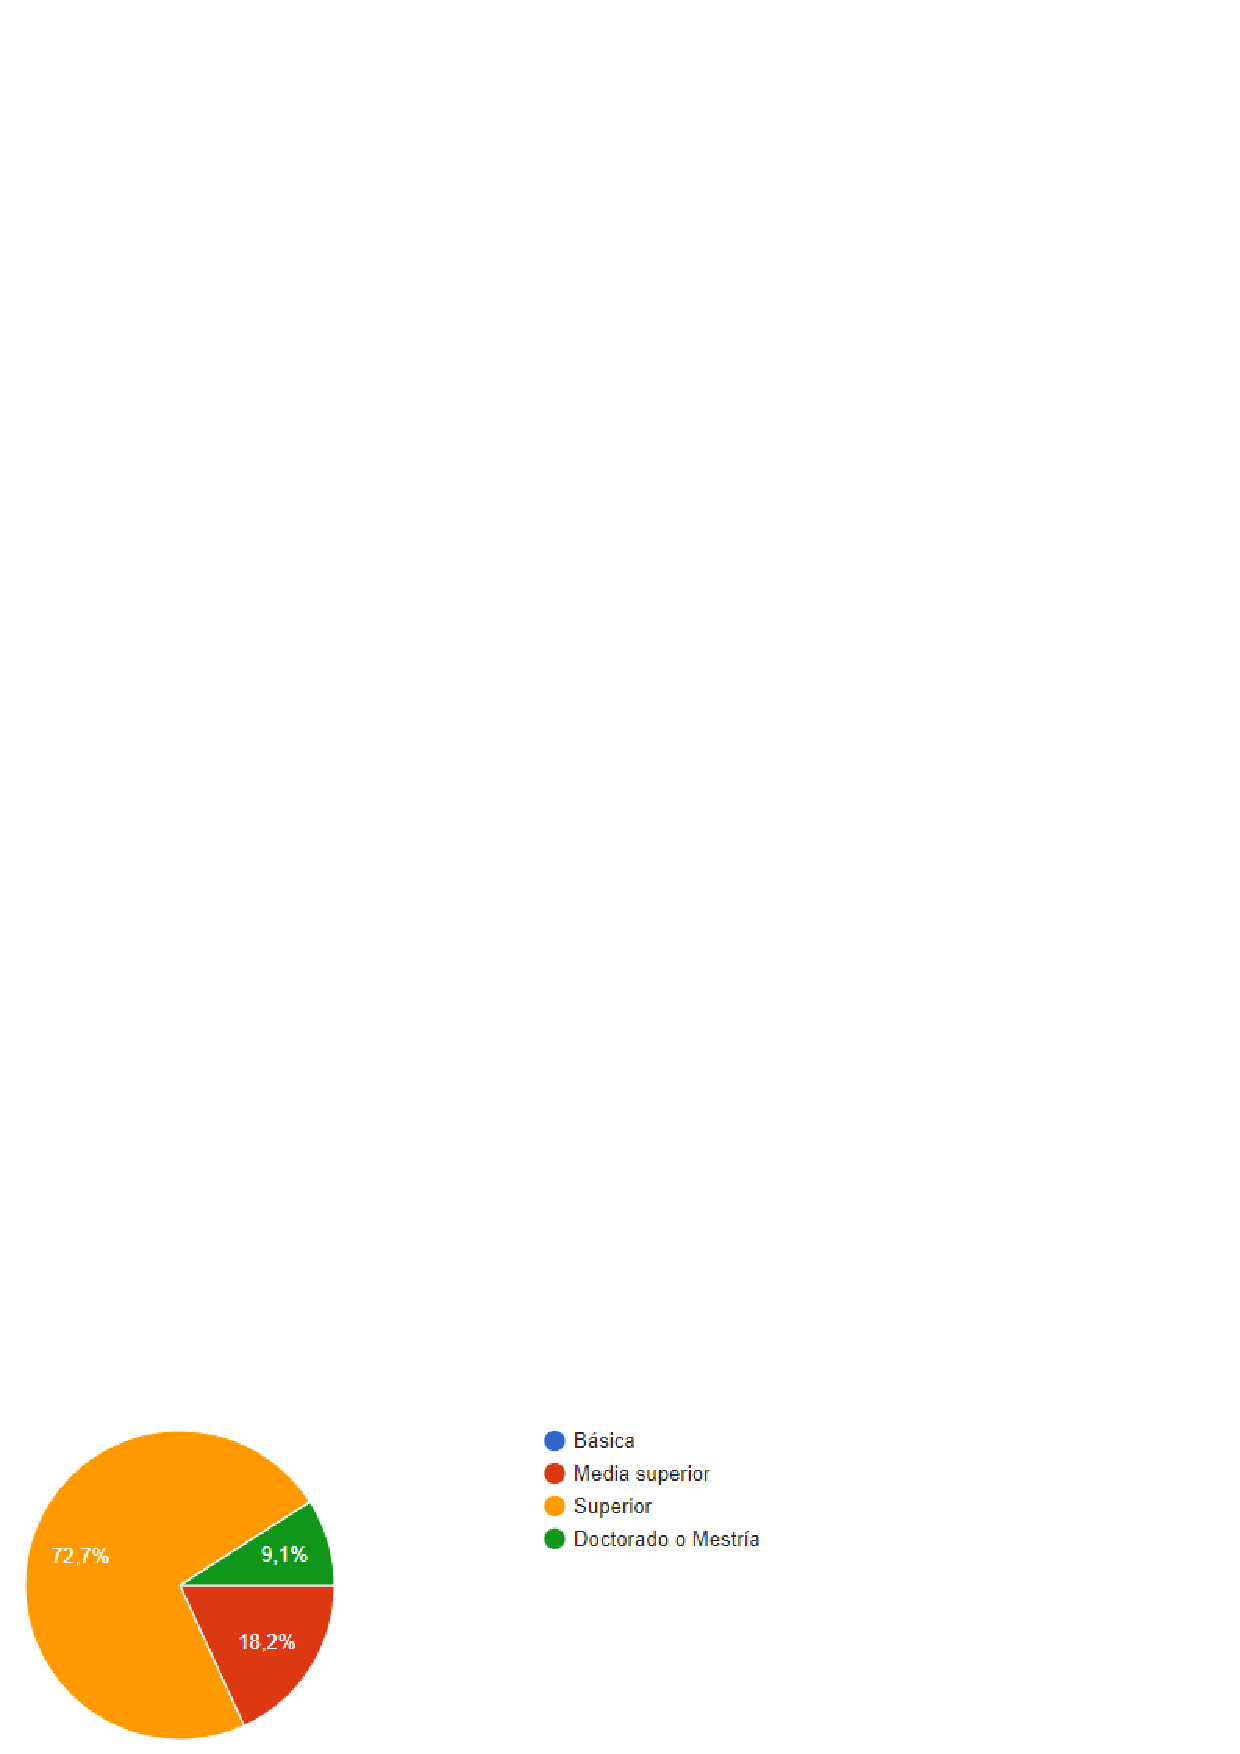
\includegraphics[width=0.5\textwidth]{04ResultadosObetnidos/pruebaR/imagenes/que/pre01}
\end{figure}

	
	 Pirámide emocional. ¿En que escalón te encuestras ahora?
	%%poner imagen
	La emoción que tenían los encuestados en ese momento era un estado de seguridad o tranquilidad.
	
	


\subsubsection{Post-juego}

	
 changing checkbox style locally
	¿Hay algún elemento que no reconozcas  o sepas que es?
	\begin{itemize}
		\item Items
		\item Personajes
		\item Fondo
		\item Texto (palabra)
		\item Lugar
		\item Tiempo
		\item Forma
		\item Otro?
	\end{itemize}

Respuesta: Los encuestados en su mayoría no reconocian diferentes formas o imágenes de objetos presentados en el juego.	

	¿Cómo califica la velocidad de reacción de los botones?
	\begin{itemize}
		\item Mala
		\item Regular
		\item Buena
	\end{itemize}

\begin{figure}
	\centering
	\caption{Gráfica de velocidad de botoness}
	\label{fig:pos01}
	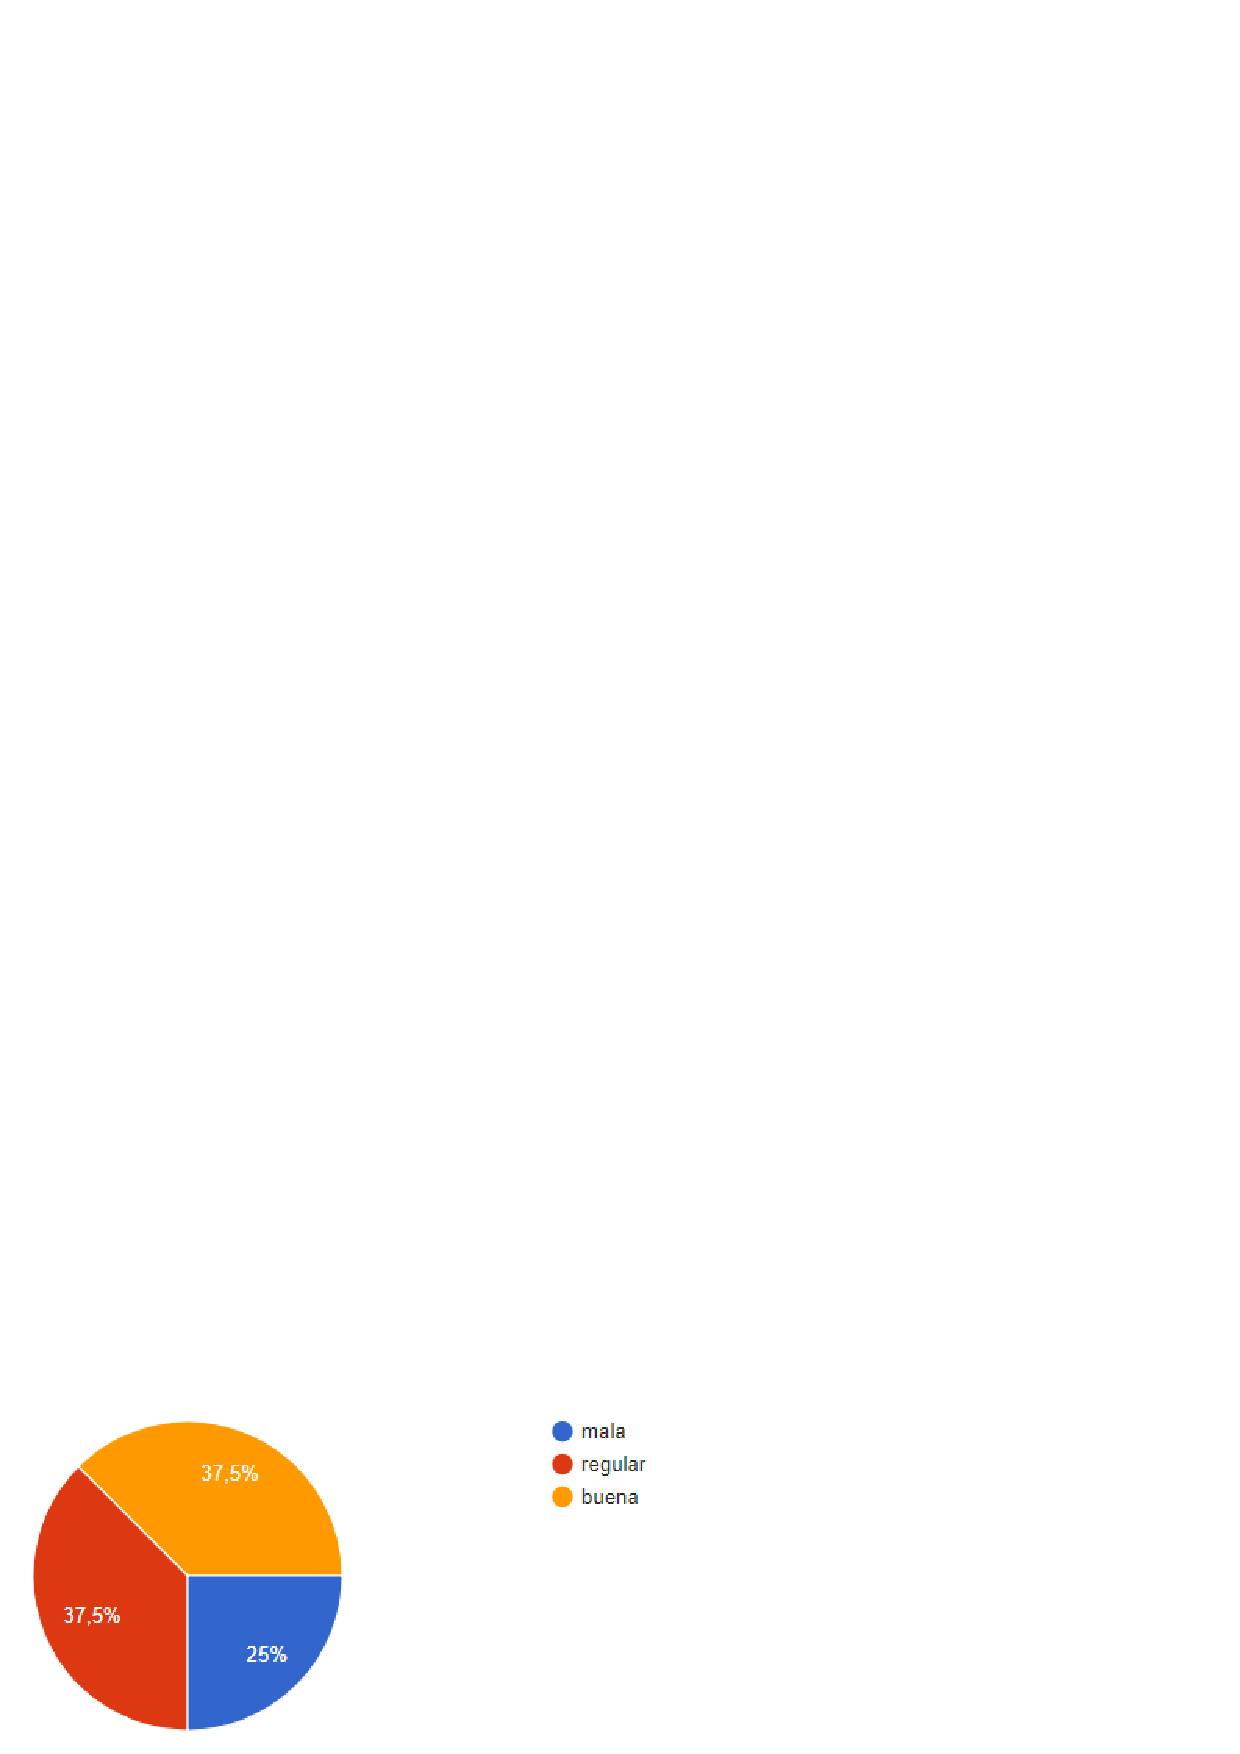
\includegraphics[width=0.5\textwidth]{04ResultadosObetnidos/pruebaR/imagenes/que/pos01}
\end{figure}

 ¿Qué te ha gustado MENOS del juego?
	\begin{itemize}
		\item Juego
		\item Dibujo
		\item Historia
		\item Temática
		\item Plataforma
	\end{itemize}

\begin{figure}
	\centering
	\caption{Gráfica de menos gusto}
	\label{fig:pos02}
	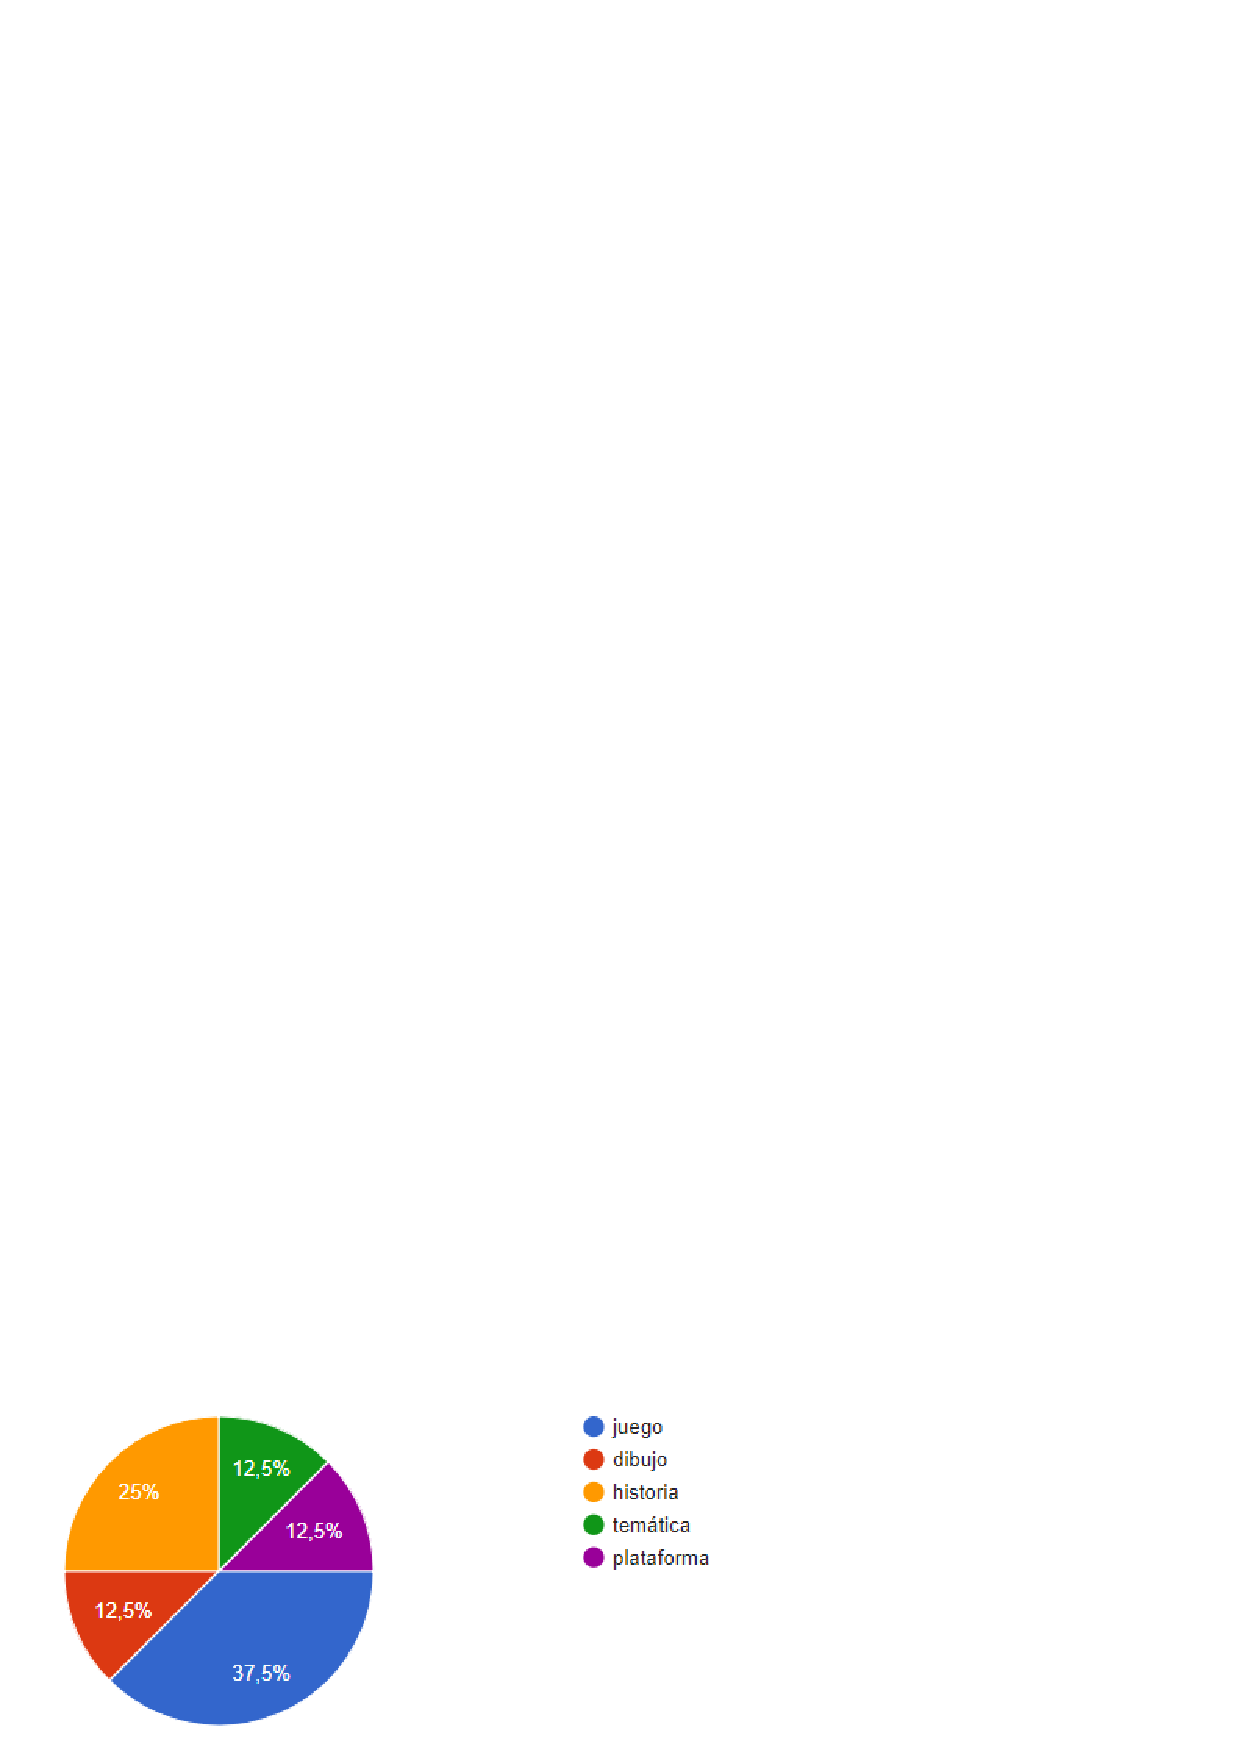
\includegraphics[width=0.5\textwidth]{04ResultadosObetnidos/pruebaR/imagenes/que/pos02}
\end{figure}

	
	¿Qué te ha gustado MÁS del juego?
\begin{itemize}
	\item Juego
	\item Dibujo
	\item Historia
	\item Temática
	\item Plataforma
\end{itemize}

\begin{figure}
	\centering
	\caption{Gráfica de más gusto}
	\label{fig:pos03}
	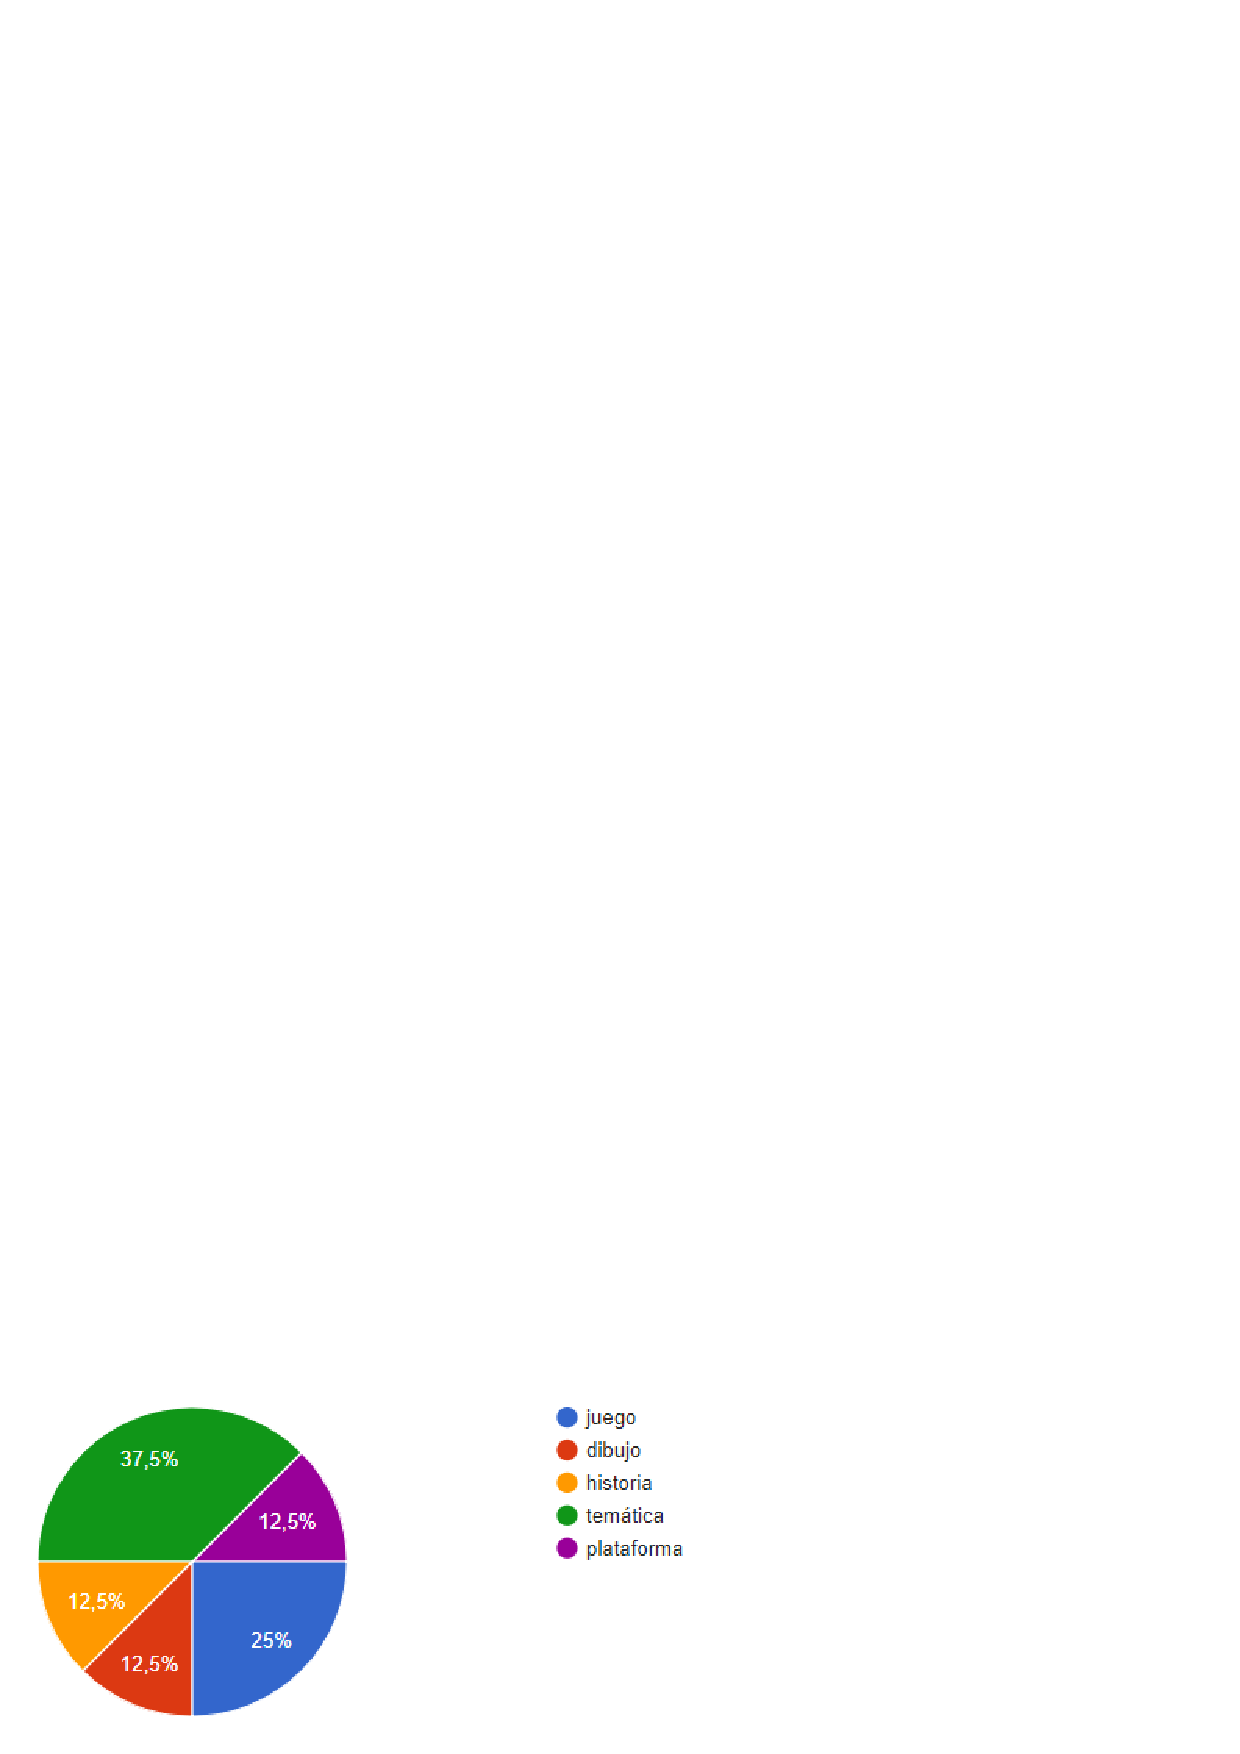
\includegraphics[width=0.5\textwidth]{04ResultadosObetnidos/pruebaR/imagenes/que/pos03}
\end{figure}


	 ¿Qué dificultad encontraste al jugar?
	Respuesta: Los encuestados en su mayoría contestaron sobre los movimientos o acciones que se podían realizar dentro del juego, que asu percepción parecían aveces impredecibles.

 ¿Que cambiarías del juego?
	Respuesta: Los usuarios en su mayoria mencionan sobre una mayor interacción en el juego sobre el personaje a otras acciones o eventos. 
	

	¿Qué senimiento tienes? 
	\begin{itemize}
		\item Alegría
		\item Enojo
		\item Tristeza
		\item Curiosidad
		\item Fatiga
		\item Otro?
	\end{itemize}

\begin{figure}
	\centering
	\caption{Gráfica de sentimiento}
	\label{fig:pos04}
	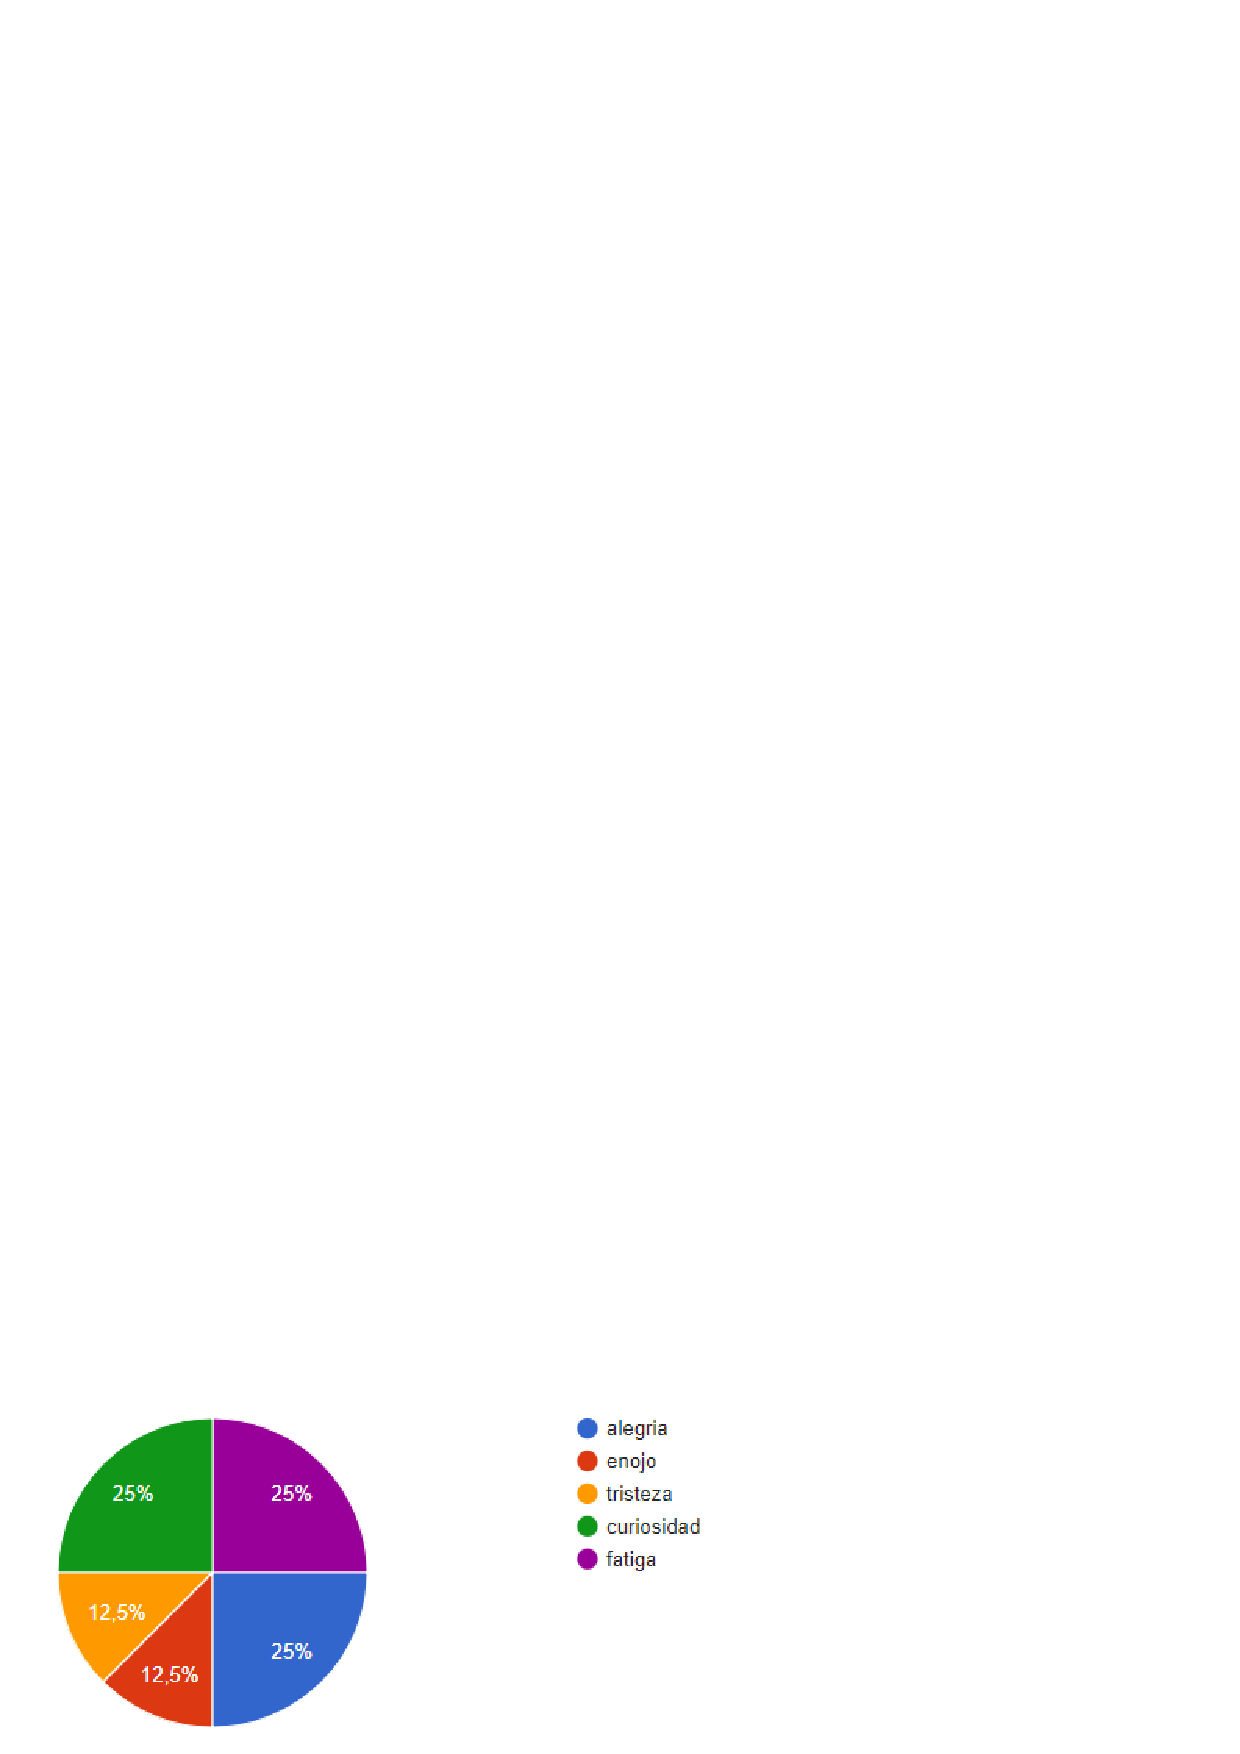
\includegraphics[width=0.5\textwidth]{04ResultadosObetnidos/pruebaR/imagenes/que/pos04}
\end{figure}



	Pirámide emocional. ¿En que escalón te encuestras ahora?
	%%poner imagen
	Respuesta: La mayoría de los jugadores seguía en el estado de seguridad o tranquilidad después del juego y seguidos de ellos algunos presentaban una emoción de autorrealización.

